\documentclass[border=5pt]{standalone}
\usepackage[T1]{fontenc}
\usepackage{lmodern}
\usepackage{tikz}
\usetikzlibrary{positioning, arrows.meta, fit, backgrounds, calc, decorations.pathreplacing, patterns}

% Colors per layer
\definecolor{dclbg}{HTML}{dbe4ff}
\definecolor{dclstroke}{HTML}{4a9eed}
\definecolor{cslbg}{HTML}{d3f9d8}
\definecolor{cslstroke}{HTML}{22c55e}
\definecolor{fslbg}{HTML}{fff3bf}
\definecolor{fslstroke}{HTML}{d4a843}
\definecolor{conflictbg}{HTML}{ffc9c9}
\definecolor{conflictstroke}{HTML}{ef4444}
\definecolor{okgreen}{HTML}{b2f2bb}
\definecolor{inputblue}{HTML}{a5d8ff}
\definecolor{inputgreen}{HTML}{c3fae8}
\definecolor{inputamber}{HTML}{ffd8a8}
\definecolor{govpurple}{HTML}{8b5cf6}
\definecolor{darkgray}{HTML}{555555}

\tikzset{
  % Node styles
  dclnode/.style={draw=dclstroke, fill=dclbg, rounded corners=4pt, font=\small\sffamily, minimum height=6mm, inner sep=3pt},
  cslnode/.style={draw=cslstroke, fill=cslbg, rounded corners=4pt, font=\small\sffamily, minimum height=12mm, inner sep=4pt, text width=25mm, align=center},
  fslok/.style={draw=cslstroke, fill=okgreen, rounded corners=4pt, font=\small\sffamily, minimum height=10mm, inner sep=3pt, align=center},
  fslsub/.style={draw, rounded corners=3pt, fill=white, font=\scriptsize\ttfamily, inner sep=3pt, align=left, minimum width=18mm},
  % Input/output boxes
  inputbox/.style={rounded corners=6pt, font=\small\sffamily, minimum width=28mm, inner sep=4pt, align=center, text width=26mm},
  outputbox/.style={rounded corners=6pt, font=\small\sffamily, minimum width=38mm, inner sep=4pt, align=center, text width=36mm},
  % Arrows
  trace/.style={-{Stealth[length=3pt]}, dashed, gray, thin},
  constraint/.style={dashed, conflictstroke, thick},
  govarrow/.style={-{Stealth[length=4pt]}, thick},
  bridge/.style={-{Stealth[length=3pt]}, thick},
}

\begin{document}
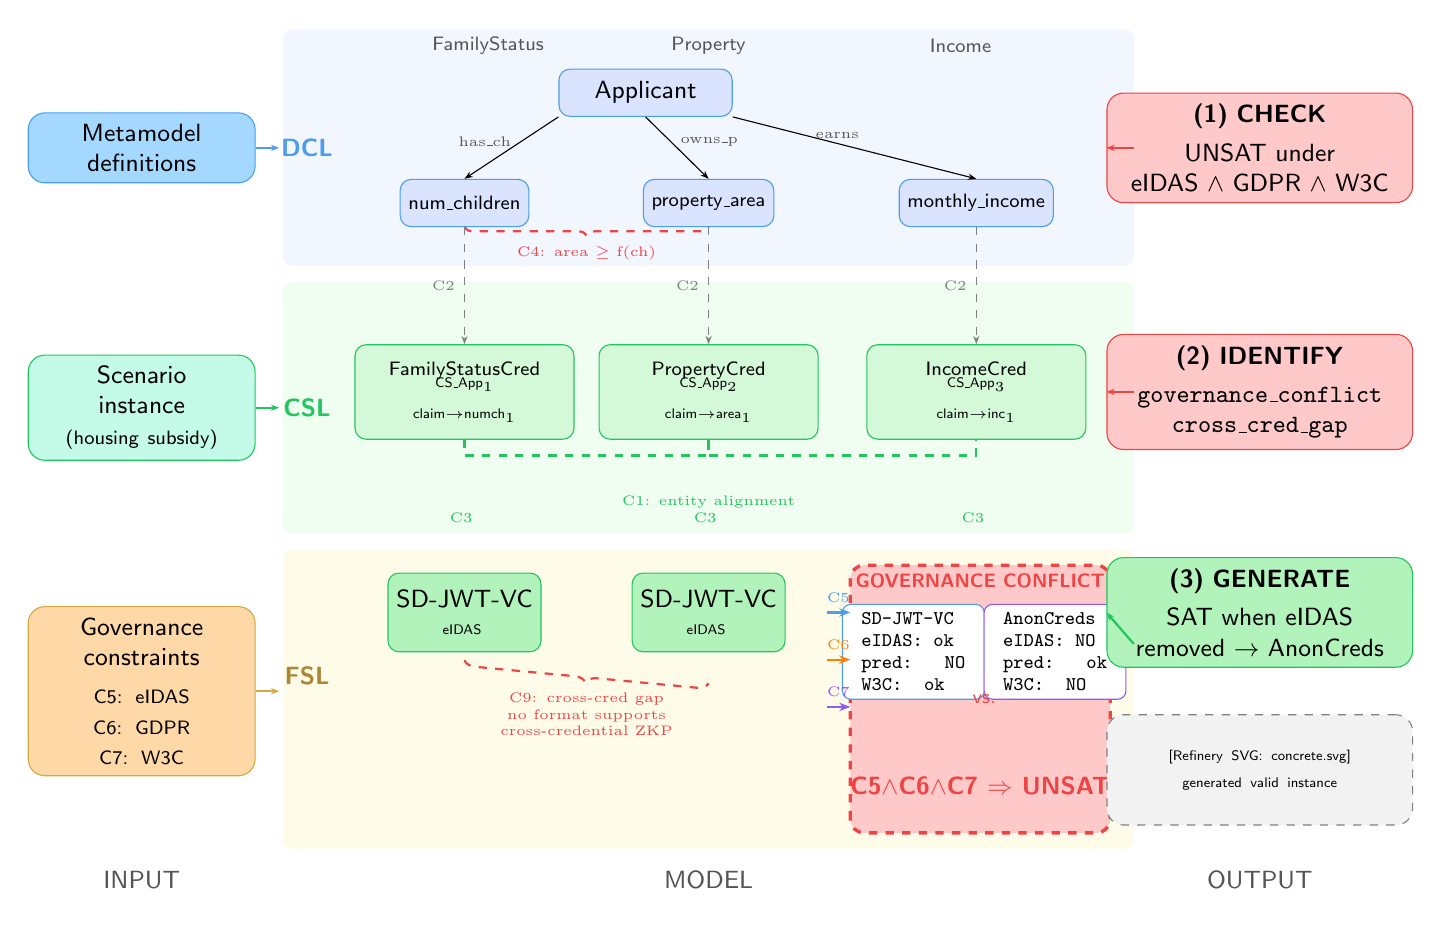
\begin{tikzpicture}[x=1mm, y=1mm]

% ============================================================
% BACKGROUND ZONES (three layer bands)
% ============================================================
\fill[dclbg, opacity=0.35, rounded corners=3pt] (32,52) rectangle (140,82);
\fill[cslbg, opacity=0.35, rounded corners=3pt] (32,18) rectangle (140,50);
\fill[fslbg, opacity=0.35, rounded corners=3pt] (32,-22) rectangle (140,16);

% Layer labels
\node[font=\small\sffamily\bfseries, color=dclstroke] at (35,67) {DCL};
\node[font=\small\sffamily\bfseries, color=cslstroke] at (35,34) {CSL};
\node[font=\small\sffamily\bfseries, color=fslstroke!80!black] at (35,0) {FSL};

% Column headers
\node[font=\scriptsize\sffamily, color=darkgray] at (58,80) {FamilyStatus};
\node[font=\scriptsize\sffamily, color=darkgray] at (86,80) {Property};
\node[font=\scriptsize\sffamily, color=darkgray] at (118,80) {Income};

% ============================================================
% INPUT COLUMN (left)
% ============================================================
\node[inputbox, draw=dclstroke, fill=inputblue] (inmeta) at (14,67) {Metamodel\\definitions};
\node[inputbox, draw=cslstroke, fill=inputgreen] (ininst) at (14,34) {Scenario\\instance\\{\scriptsize(housing subsidy)}};
\node[inputbox, draw=fslstroke, fill=inputamber, text width=26mm] (ingov) at (14,-2) {Governance\\constraints\\[1mm]{\scriptsize C5: eIDAS}\\{\scriptsize C6: GDPR}\\{\scriptsize C7: W3C}};

% Arrows from inputs to model zones
\draw[bridge, dclstroke] (inmeta.east) -- ++(3,0);
\draw[bridge, cslstroke] (ininst.east) -- ++(3,0);
\draw[bridge, fslstroke] (ingov.east) -- ++(3,0);

% ============================================================
% DCL CONTENT
% ============================================================
\node[dclnode, minimum width=22mm] (app) at (78,74) {Applicant};

\node[dclnode] (numch) at (55,60) {\scriptsize num\_children};
\node[dclnode] (proparea) at (86,60) {\scriptsize property\_area};
\node[dclnode] (moninc) at (120,60) {\scriptsize monthly\_income};

\draw[-{Stealth[length=3pt]}] (app.south west) -- node[left, font=\tiny, color=darkgray, pos=0.4] {has\_ch} (numch.north);
\draw[-{Stealth[length=3pt]}] (app.south) -- node[right, font=\tiny, color=darkgray, pos=0.4] {owns\_p} (proparea.north);
\draw[-{Stealth[length=3pt]}] (app.south east) -- node[right, font=\tiny, color=darkgray, pos=0.3] {earns} (moninc.north);

% C4 constraint arc
\draw[constraint, decoration={brace, mirror, amplitude=3pt}, decorate]
  (numch.south) -- (proparea.south)
  node[midway, below=3pt, font=\tiny, color=conflictstroke] {C4: area $\geq$ f(ch)};

% ============================================================
% CSL CONTENT
% ============================================================
\node[cslnode] (cfam) at (55,36) {\scriptsize FamilyStatusCred\\[-0.5mm]\tiny CS\_App$_1$\\claim$\to$numch$_1$};
\node[cslnode] (cprop) at (86,36) {\scriptsize PropertyCred\\[-0.5mm]\tiny CS\_App$_2$\\claim$\to$area$_1$};
\node[cslnode] (cinc) at (120,36) {\scriptsize IncomeCred\\[-0.5mm]\tiny CS\_App$_3$\\claim$\to$inc$_1$};

% C2: trace arrows
\draw[trace] (numch.south) -- (cfam.north) node[midway, left, font=\tiny, color=gray] {C2};
\draw[trace] (proparea.south) -- (cprop.north) node[midway, left, font=\tiny, color=gray] {C2};
\draw[trace] (moninc.south) -- (cinc.north) node[midway, left, font=\tiny, color=gray] {C2};

% C1: entity alignment arc
\draw[dashed, cslstroke, thick]
  (cfam.south) -- ++(0,-2) -| (cprop.south)
  node[midway, below=0pt, font=\tiny, color=cslstroke] {};
\draw[dashed, cslstroke, thick]
  (cprop.south) -- ++(0,-2) -| (cinc.south);
\node[font=\tiny, color=cslstroke] at (86,22) {C1: entity alignment};

% C3: non-empty markers
\node[font=\tiny, color=cslstroke] at (55,20) {C3 $\checkmark$};
\node[font=\tiny, color=cslstroke] at (86,20) {C3 $\checkmark$};
\node[font=\tiny, color=cslstroke] at (120,20) {C3 $\checkmark$};

% ============================================================
% FSL CONTENT
% ============================================================

% OK format boxes
\node[fslok] (sdjwt1) at (55,8) {SD-JWT-VC\\[-0.5mm]{\tiny eIDAS $\checkmark$}};
\node[fslok] (sdjwt2) at (86,8) {SD-JWT-VC\\[-0.5mm]{\tiny eIDAS $\checkmark$}};

% ============================================================
% CONFLICT ZONE
% ============================================================
\draw[conflictstroke, very thick, dashed, fill=conflictbg, rounded corners=5pt]
  (104,-20) rectangle (137,14);

\node[font=\scriptsize\sffamily\bfseries, color=conflictstroke] at (120.5,12) {GOVERNANCE CONFLICT};

% Two sub-boxes showing the dilemma
\node[fslsub, draw=dclstroke] (sub1) at (112,3) {SD-JWT-VC\\eIDAS: \textbf{ok}\\pred:\;\; \textbf{NO}\\W3C:\;\; \textbf{ok}};
\node[fslsub, draw=govpurple] (sub2) at (130,3) {AnonCreds\\eIDAS: \textbf{NO}\\pred:\;\; \textbf{ok}\\W3C:\;\; \textbf{NO}};

\node[font=\scriptsize\sffamily, color=conflictstroke] at (121,-3) {vs.};

% UNSAT label
\node[font=\small\sffamily\bfseries, color=conflictstroke] at (120.5,-14) {C5$\wedge$C6$\wedge$C7 $\Rightarrow$ UNSAT};

% Governance convergence arrows (C5, C6, C7 entering conflict zone)
\draw[govarrow, dclstroke] (101,8) -- (104,8) node[midway, above, font=\tiny] {C5};
\draw[govarrow, orange] (101,2) -- (104,2) node[midway, above, font=\tiny] {C6};
\draw[govarrow, govpurple] (101,-4) -- (104,-4) node[midway, above, font=\tiny] {C7};

% C9: cross-credential predicate gap
\draw[constraint, decoration={brace, mirror, amplitude=4pt}, decorate]
  (sdjwt1.south) ++(0,-1) -- (sdjwt2.south |- 0,-1)
  node[midway, below=4pt, font=\tiny, color=conflictstroke, text width=35mm, align=center]
  {C9: cross-cred gap\\no format supports\\cross-credential ZKP};

% ============================================================
% OUTPUT COLUMN (right)
% ============================================================
\node[outputbox, draw=conflictstroke, fill=conflictbg] (ochk) at (156,67)
  {\textbf{(1) CHECK}\\[1mm]UNSAT under\\eIDAS $\wedge$ GDPR $\wedge$ W3C};

\node[outputbox, draw=conflictstroke, fill=conflictbg] (oid) at (156,36)
  {\textbf{(2) IDENTIFY}\\[1mm]{\small\texttt{governance\_conflict}}\\{\small\texttt{cross\_cred\_gap}}};

\node[outputbox, draw=cslstroke, fill=okgreen] (ogen) at (156,8)
  {\textbf{(3) GENERATE}\\[1mm]SAT when eIDAS\\removed $\to$ AnonCreds};

% Refinery SVG placeholder
\node[outputbox, draw=gray, dashed, fill=black!5, text width=36mm, minimum height=14mm] (svgph) at (156,-12)
  {{\tiny [Refinery SVG: concrete.svg]}\\[-0.5mm]{\tiny generated valid instance}};

% Leader arrows from model to output
\draw[bridge, conflictstroke] (140,67) -- (ochk.west);
\draw[bridge, conflictstroke] (140,36) -- (oid.west);
\draw[bridge, cslstroke] (140,4) -- (ogen.west);

% ============================================================
% BOTTOM LABELS
% ============================================================
\node[font=\small\sffamily, color=darkgray] at (14,-26) {INPUT};
\node[font=\small\sffamily, color=darkgray] at (86,-26) {MODEL};
\node[font=\small\sffamily, color=darkgray] at (156,-26) {OUTPUT};

\end{tikzpicture}
\end{document}
